\documentclass{report}
\usepackage{graphicx}
\usepackage{listings}
\usepackage{color}
\usepackage[margin=1.2in]{geometry}
\usepackage{courier}
\usepackage{float}
\usepackage[toc,page]{appendix}
\usepackage{hyperref}

\definecolor{codegreen}{rgb}{0,0.6,0}
\definecolor{codeblack}{rgb}{0,0,0}
\definecolor{codered}{rgb}{0.867,0,0}
\definecolor{backcolour}{rgb}{ 0.95,0.95,0.95}
\definecolor{codeorange}{rgb}{1,0.447059,0}
\definecolor{codegrey}{rgb}{0.1, 0.1, 0.1}
\definecolor{codeblue}{rgb}{0.29, 0.52, 0.56}
\lstdefinestyle{mystyle}{
    basicstyle=\ttfamily\color{codeblack},
    backgroundcolor=\color{backcolour},   
    commentstyle=\color{codered},
    keywordstyle=\color{codeorange},
    numberstyle=\color{codeblack},
    stringstyle=\color{codegreen},
    breakatwhitespace=false,         
    breaklines=true,                 
    captionpos=b,                    
    keepspaces=true,                 
    numbers=left,                    
    numbersep=10pt,                  
    showspaces=false,                
    showstringspaces=false,
    showtabs=false,                  
    tabsize=2
}
 
\lstset{style=mystyle}

\newcommand{\ul}[1]{\underline{#1}}
\newcommand{\ull}[1]{\underline{\underline{#1}}}
\newcommand{\triangleBrac}[1]{\textless{#1}\textgreater}
\newcommand{\un}{\textunderscore}

\begin{document}
\title{CPS2000  - Compiler Theory and Practice - Assignment Report}
\author{Daniel Cauchi}
\date{}
\maketitle

\tableofcontents

\chapter{Introduction}
This is the report for the CPS2000 Compilers assignment, where a compiler and interpreter for the MiniLang programming language was created, with a Lexer, Parser, XML generator, Semantic Analyser and Interpreter. The C++ programming language was used in conjunction with the VSCode IDE. The program was tested on the Linux Subsystem for Windows and C++11 was used, using the provided CMakeLists.txt. It works without any known errors and any compiler warnings were dealt with. A video showcase is also linked (in the README) to show the compiler in action, with several input files to show different aspects of it working in proper order. Every part of the assignment was tackled and shown to be functioning appropriately.

A description and example for each of the tasks is given in chapter 2 of this report. The code is divided into folders to categorize them by their functionality. Any error in any input file is also given appropriately, with specified line number, with the limitation that only one error at a time may be displayed.

\chapter{Tasks}
\section{Task 1 - Lexer}
\subsection{Explanation and Implementation}
The Lexer tokenizes the input stream by taking in character by character, grouping then into ordered tokens. A token is a tuple of (Lexeme, Attribute).

The following transition groups fo the characters were chosen (This is also the Classifier Table):
\begin{enumerate}
	\item Singular punctuation (punctuation which exists on its own): + - ( ) \textbraceleft \textbraceright ; $\colon$ ,
	\item Exclamation point: !
	\item Fullstop: .
	\item Digit: 0-9
	\item Alpha: A-Z a-z \textunderscore
	\item Forward slash: /
	\item New-line: \textbackslash n
	\item Asterisk: *
	\item Equals: =
	\item Whitespace/tab or \textbackslash r: ' ' \textbackslash t \textbackslash r
	\item Greater/Smaller than: \textless  \textgreater
	\item Other: anything else
\end{enumerate}

The following diagram is the state transition diagram DFA. Note: 'not X' means any other character which is not X.
\begin{figure}[H]
	\centering
	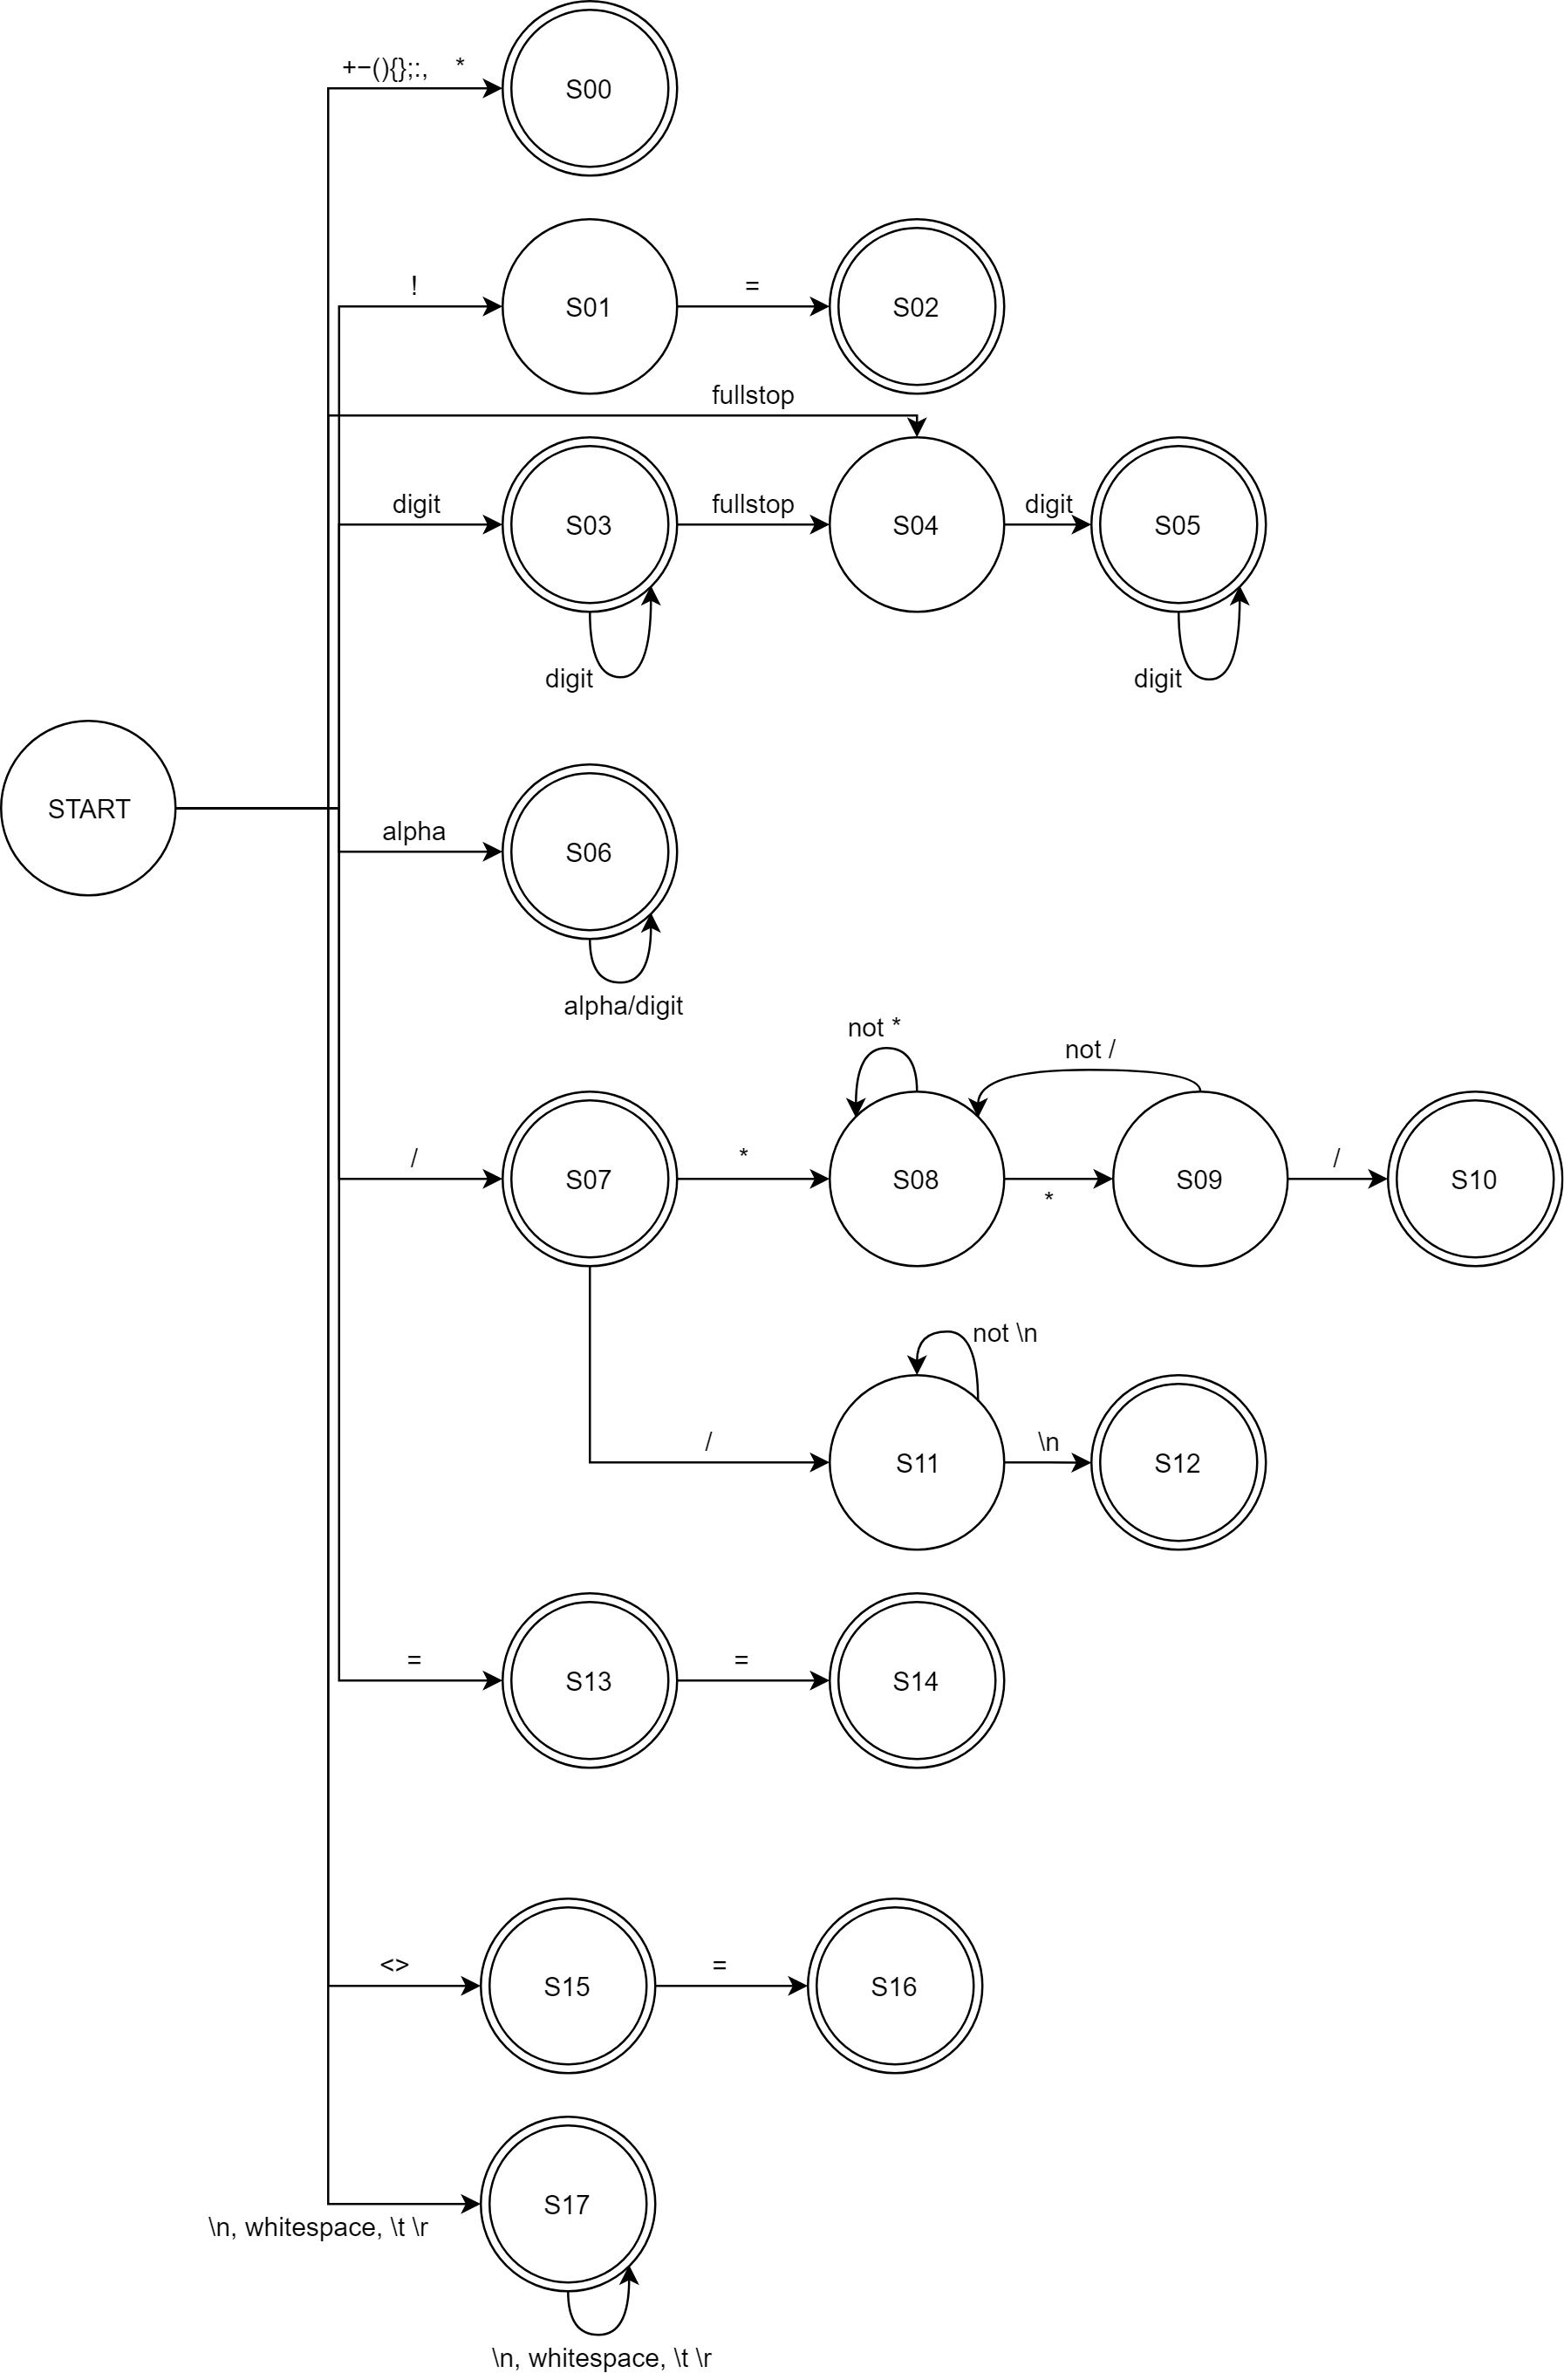
\includegraphics[scale=0.22]{Images/Q1_StateTransitionDiagram.png}
	\caption{DFA for Lexer}
\end{figure}

As a table, it looks like this in the code. The comments help to understand it better \cite{StateTransitionTable}:
\begin{figure}[H]
	\centering
	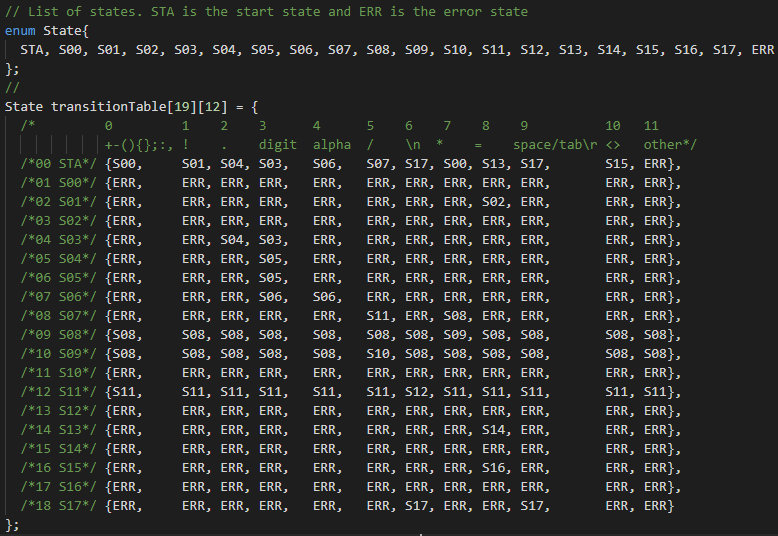
\includegraphics[width=\textwidth]{Images/Q1_StateTransitionTable.PNG}
	\caption{Table for Lexer}
\end{figure}

If the program goes to ERR (the error state), then the lexeme is over. If the current state is not a final state, then an error is reported and Lexical Analysis stops. If if the program goes to ERR and is in a final state, then the lexeme is kept and tokenized.

The token class is the following (Found in the Token.h file):
\begin{lstlisting}[language=C++]
class Token{
	public:
		static string TokenString[]; // Stings corresponding to the enum of token types
		enum TokenType{
		ID, BOOL, FLOAT, INT, // ID and constants
		ST, SE, GT, GE, EQQ, NE, AND, OR, NOT, // conditional operators
		EQ, PLUS, MINUS, TIMES, DIVISION, //arithmetic operators
		IF, ELSE, FOR, WHILE, FN, RETURN, TYPE_BOOL, TYPE_FLOAT, TYPE_INT, VAR, //keywords
		COLON, SEMI_COLON, COMMA, //punctuation
		OPEN_BRACKET, CLOSED_BRACKET, OPEN_BRACE, CLOSED_BRACE, //brackets punctuation
		COMMENT
		};
		
		// the Token parameters
		TokenType type;
		string lexeme = "";
		float number;
		
		// constructor
		Token (TokenType _type, string _lexeme, float _number){
		type = _type;
		lexeme = _lexeme;
		number = _number;
}

// helper method to neatly print the current token
void printToken();
};
\end{lstlisting}

The final states result in some token. The following is a list of which states can result to which tokens (based on the lexeme).
\begin{enumerate}
	\item S0: PLUS, OPEN\textunderscore BRACKET, CLOSED\textunderscore BRACKET, OPEN\textunderscore BRACE, CLOSED\textunderscore BRACE, COLON, SEMI\textunderscore COLON, COMMA, TIMES
	\item S2: NE
	\item S3: INT
	\item S5: FLOAT
	\item S6: ID (or one of mykeywords[] below)
	\item S7: DIVISION
	\item S11: discard '/*' and '*/' and return COMMENT
	\item S13: discard '//' and return COMMENT
	\item S14: EQ
	\item S15: EQQ
	\item S16: GT, ST
	\item S17: GE, SE
	\item S18: discard, since it is white spaces or new lines or tabs or carriage returns only
\end{enumerate}

\bigskip

The array of keywords in Token.cpp is as follows:
\begin{lstlisting} [language=C++]
// Used to check if a given string is a keyword (or identifier), and what type of keyword it is
struct keyword_token{
	string text;
	Token::TokenType tok_type;
};

keyword_token my_keywords[] = {
	{"and", Token::AND},
	{"or", Token::OR},
	{"not", Token::NOT},
	{"if", Token::IF},
	{"else", Token::ELSE},
	{"for", Token::FOR},
	{"while", Token::WHILE},
	{"fn", Token::FN},
	{"return", Token::RETURN},
	{"bool", Token::TYPE_BOOL},
	{"float", Token::TYPE_FLOAT},
	{"int", Token::TYPE_INT},
	{"var", Token::VAR},
	{"true", Token::BOOL},
	{"false", Token::BOOL}
};
\end{lstlisting}

The Lexer's \textit{Lex()} function does the following:
\begin{enumerate}
	\item Initialise state to the start state
	\item Initialise lexeme to the empty string
	\item Until EOF:
	\item \quad Read next character from the file
	\item \quad See to which column in the table this character points to, and use the current state as the row value to go to the new state
	\item \quad If at en error state
	\item \quad \quad Check if the the lexeme is valid with the previous state before the error state. If it is invalid, report the error, otherwise reset the lexeme and the state and go to step 3
	\item \quad else set the state as the one obtained from step 5 as the next state and append the character to the lexeme. Go back to step 3
\end{enumerate}

\subsection{Example Test}
Using the \textit{printToken()} in the \textit{Token} class \textit{printTokens()} method in the \textit{Lexer} class, when the following input is given to the program:
\begin{lstlisting}
someid true false 12.3 .4 56 89
< <= > >= == != and or not
= + - * /
if else for while fn return bool float int var
: ; ,
() {}
// hello world
/* hello 
world
2 */
\end{lstlisting}
The following output is printed from \textit{printTokens()}

\begin{figure}[H]
	\centering
	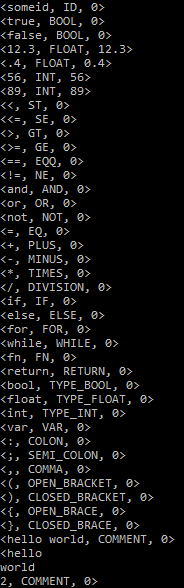
\includegraphics[scale=1]{Images/Q1_ExampleTest.png}
	\caption{Example output for the example input}
\end{figure}


\pagebreak
\section{Task 2 - Parser}
\subsection{Explanation and Implementation}

The parser takes the tokens and puts them into a parse tree based on the grammar. The following is the grammar re-written to make terminals and non terminals more visible. Terminals are underlined while non-terminals are enclosed in brackets. Square brackets represent optional parts while curly braces represent parts which may be repeated. The peeking method is used whenever there is the use of options(sub-bullet points, which represent $|$), [] or \{\}, this is done in order to \textbf{avoid back-tracking}. The parser uses something close to the FIRST set in order to peek as much as it needs to, so as to determine the next production to choose. Note: An identifier non-terminal was created due to 'Factor', since it accepts a node, so ID was enclosed within a non-terminal.

\begin{itemize}
	\item Type
		\subitem \ul{TYPE\un FLOAT}
		\subitem \ul{TYPE\un INT}
		\subitem \ul{TYPE\un BOOL}
	\item Literal
		\subitem \ul{FLOAT}
		\subitem \ul{INT}
		\subitem \ul{BOOL}
	\item Identifier
		\subitem \ul{ID}
	\item MultiplicativeOp
		\subitem \ul{TIMES}
		\subitem \ul{DIVISION}
		\subitem \ul{AND}
	\item AdditiveOp
		\subitem \ul{PLUS}
		\subitem \ul{MINUS}
		\subitem \ul{OR}
	\item ReltionalOp
		\subitem \ul{ST}
		\subitem \ul{GT}
		\subitem \ul{EQQ}
		\subitem \ul{NE}
		\subitem \ul{SE}
		\subitem \ul{GE}
	\item ActualParams
		\subitem (Expression) \{ \ul{COMMA} (Expression) \}
	\item FunctionCall
		\subitem (Identifier) \ul{OPEN\un BRACKET} [(ActualParams)] \ul{CLOSED\un BRACKET}
	\item SubExpression 
		\subitem \ul{OPEN\un BRACKET} (Expression) \ul{CLOSED\un BRACKET}
	\item Unary
		\subitem \ul{MINUS} (Expression)
		\subitem \ul{NOT} (Expression)
	\item Factor
		\subitem (Literal)
		\subitem (Identifier)
		\subitem (FunctionCall)
		\subitem (SubExpression)
		\subitem (Unary)
	\item Term
		\subitem (Factor) \{ (MultiplicativeOp) (Factor) \}
	\item SimpleExpression
		\subitem (Term) \{ (AdditiveOp) (Term) \}
	\item Expression
		\subitem (SimpleExpression) \{ (RelationalOp) (SimpleExpression) \}
	\item Assignment
		\subitem (Identifier) \ul{EQUALS} (Expression)
	\item VariableDecl
		\subitem \ul{VAR} (Identifier) \ul{COLON} (Type)	\ul{EQ} (Expression)
	\item PrintStatement
		\subitem \ul{PRINT} (Expression)
	\item ReturnStatement
		\subitem \ul{RETURN} (Expression)
	\item IfStatement
		\subitem \ul{IF} \ul{OPEN\un BRACKET} (Expression) \ul{CLOSED\un BRACKET} (Block) [ \ul{ELSE} (Block) ]
	\item ForStatement
		\subitem \ul{FOR} \ul{OPEN\un BRACKET} [ (VariableDecl) ] \ul{SEMI\un COLON} (Expression) \ul{SEMI\un COLON} [ (Assignment) ] \ul{CLOSED\un BRACKET} (Block)
	\item FormalParam
		\subitem (Identifier) \ul{COLON} (Type)
	\item FormalParams
		\subitem \ul{FormalParam} \{ \ul{COMMA} (FormalParam) \}
	\item FunctionDecl
		\subitem \ul{FN} (Identifier) \ul{OPEN\un BRACKET} [ (FormalParams) ] \ul{CLOSED\un BRACKET} \ul{COLON} (Type) (Block)
	\item Statement
		\subitem (VariableDecl) \ul{SEMI\un COLON}
		\subitem (Assignment) \ul{SEMI\un COLON}
		\subitem (PrintStatement) \ul{SEMI\un COLON}
		\subitem (IfStatement)
		\subitem (ForStatement)
		\subitem (ReturnStatement) \ul{SEMI\un COLON}
		\subitem (FunctionDecl)
		\subitem (Block)
	\item Block
		\subitem \ul{OPEN\un BRACE} \{ Statement \} \ul{CLOSED\un BRACE}
	\item Program
		\subitem \{ (Statement) \}
\end{itemize}

Since it is an Abstract Syntax tree, the following tokens are matched and immediately discarded by the parser: OPEN\un BRACKET, CLOSED\un BRACKET, OPEN\un BRACE, CLOSED \un BRACE, SEMI\un COLON, COLON, COMMA, FN, VAR, RETURN, IF, ELSE, FOR, PRINT

From the above, it is shown that there are 25 possible types of nodes. This is because the tree is not fully abstract. The advantage of this is that operator precedence for expressions is handled automatically by the grammar, while the disadvantage is that it leads to more complexity, since each type of node needs to be catered for.

Regarding implementation, the \textit{Parser} class receives the tokens and stores them in a \textit{TokenManager} so that they are managed by the functions in this manager. The \textit{Parser} class also holds the root node of the recursive AST which will be generated when the \textit{parse()} method is called.

The 26 ASTNodes classes (27 counting the abstract class used for polymorphism) each have a parse method to parse their own form accordingly, and store what is parsed in their own way. For example, the \textit{Type} ASTNode, will store a token whose type is TYPE\un FLOAT, TYPE\un INT or TYPE\un BOOL. Meanwhile, a program will contain a list (vector) of statements.

Each parse method for the ASTNodes will return true or false, to tell the callback recursion whether it was successful or not. Since a predictive parser with follow sets is used, then all should return true, and if one is false, then parsing fails and the \textbf{error and the line number} is reported to the user. The function \textit{match(TokenType)} is used to check if  token is matched. It is used especially in cases where a bracket needs to be matched. If the required token type is not found, then the error that the required token was not found is reported to the user and the parser exits.
\\ \\
Taking the following parse method for ASTNodeIdentifier:
\begin{lstlisting}[language=C++]
class ASTNodeIdentifier : virtual public ASTNode{
	public:
		// costructor is same as parent
		ASTNodeIdentifier(TokenManager *tokenManager) : ASTNode(tokenManager) {};
		virtual ~ASTNodeIdentifier(){};
		virtual bool parse(); // returns true if parse was successful
		virtual void accept(Visitor *v);
		
		Token* token;
};
\end{lstlisting}

\begin{lstlisting}[language=C++]
bool ASTNodeIdentifier::parse(){
	token = match(ID);
	return true;
}
\end{lstlisting}
The process is that the token is simply stored within the variable \textit{token}, and it becomes a leaf of the tree (all leaves of the tree are tokens, while the internal nodes are ASTNodes).
\\\\
Taking a more complex example of the ASTNodeIfStatement:
\begin{lstlisting}[language=C++]
class ASTNodeIfStatement : virtual public ASTNode{
	public:
		// costructor is same as parent
		ASTNodeIfStatement(TokenManager *tokenManager) : ASTNode(tokenManager) {};
		virtual ~ASTNodeIfStatement();
		virtual bool parse(); // returns true if parse was successful
		virtual void accept(Visitor *v);
		
		ASTNode* expression;
		ASTNode* block;
		ASTNode* elseBlock = NULL; // optional
};
\end{lstlisting}

\begin{lstlisting}[language=C++]
bool ASTNodeIfStatement::parse(){
	match(IF);
	match(OPEN_BRACKET);
	
	ASTNode *n = new ASTNodeExpression(tokenManager);
	if (n->parse() == false) return false;
	expression = n;
	
	match(CLOSED_BRACKET);
	
	ASTNode *n2 = new ASTNodeBlock(tokenManager);
	if (n2->parse() == false) return false;
	block = n2;
	
	if(tokenManager->peekToken()->type == ELSE){
		match(ELSE);
		
		ASTNode *n3 = new ASTNodeBlock(tokenManager);
		if (n3->parse() == false) return false;
		elseBlock = n3;
	}
	
	return true;
}
ASTNodeIfStatement::~ASTNodeIfStatement(){
	delete expression;
	delete block;
	delete elseBlock;
}
\end{lstlisting}

The first thing to notice is that an IF statement has three children and none of them are leaves. The parse method starts by first matching an IF and OPEN\un BRACKET and discards them (lines 2 and 3), afterwards it tries to parse an ASTNodeExpression(lines 5 and 6). If it fails, the entire process returns false (line 6). Otherwise, if it is successful, the expression node within the if node is set to the newly parsed expression node. This shows how the parse method is a recursive function, until leaves are found. The rest of the method follows suit. Note how the else block is optional, so first the parser checks if it should expect an else block by checking for an ELSE token (line 15), and if it does not exists, it is skipped over, otherwise it is set accordingly.


\subsection{Example Test}
The parse method returns true or false, and it is difficult to visualise the tree, so instead a visualization of this process can be shown in the next section XMLGeneration, for a proper visualization of the tree.
\pagebreak
\section{Task 3 - XMLGeneration}
\subsection{Explanation and Implementation}


\pagebreak
\section{Task 4 - Semantic Analysis}
\subsection{Explanation and Implementation}
The task of the semantic analysis is to perform type checking and scope checking by traversing the AST and making the required checks at each node.

In order to achieve this, a new visitor inherited class was created called \textit{SAVisitor}. It contains the following functionality and data in order to perform its job (as well as the visit methods).

\begin{lstlisting}[language=C++]
vector<map<string, TokenType>> scope;
void newScope(); // add scope as the 0 index of the vector
void insert(string, TokenType); // in current scope
void removeScope(); // remove scope at position 0
// set as pointer to TokenType due to the need to make it return null
TokenType* lookup(string); // lookup starting from index 0 and going down
// a map, mapping function names to their parameter types
map <string, vector<TokenType> > functions;
TokenType currentFunctionType;
\end{lstlisting}

The scope vector is treated like a stack, but created as a vector to be iterated over easily. New entries are inserted at the front (position 0) of the vector and same thing with deletions. When iterating, iteration also starts from the front, so new entries cover shadow old ones (scope shadowing).
\\\\
Next, the visit classes are discussed. Each one of these, although described as a \textit{void*}, has some form of concrete return value, and not all of them are the same. The functionality of each method and their return type is discussed below, for each type of ASTNode visit method:
\begin{itemize}
	\item Type : Type 
		\subitem returns FLOAT, INT or BOOL(the type) depending on its token
	\item Literal : Type
		\subitem returns the type of its literal value
	\item Identifier : Type
		\subitem returns the type of its identifier obtained from the symbol table. Error if it is not found
	\item MultiplicativeOp : Operator Token (ex. TIMES, AND)
		\subitem returns the operator itself, so that the expression node it belongs to can check that the operator supports the types it is operating upon. (Ex. "7*8" is valid, but "7 and 8" is not)
	\item MultiplicativeOp : Operator Token (ex. PLUS, OR)
		\subitem very similar to MultiplicativeOp but with different operators
	\item RelationalOp : Operator Token (ex. EQQ, ST)
		\subitem very similar to MultiplicativeOp but with different operators
	\item ActualParams : Vector of Type
		\subitem iterates through all the parameters and returns a vector of all their types, so they can be matched with the formal parameters by the FunctionDecl node.
	\item FunctionCall : Type
		\subitem validates the function exists
		\subitem validates the parameters provided are of the required type
		\subitem If any of these are false, the required errors are reported and program exits
	\item SubExpression : Type
		\subitem returns the type of the expression it has
	\item Unary : Type
		\subitem validates that the unary operator is applied on the proper type and returns the type of the expression
	\item Factor : Type
		\subitem returns the type of its node	
	\item SimpleExpression : Type
		\subitem validates that any operators are being used properly and are of the correct type
		\subitem returns the type after checking and possibly performing type casting (ex. "4+6.8" returns float, while 4*true gives an error)
	\item Expression : Type
		\subitem very similar to SimpleExpression but with additive operators instead
	\item Assignment : void
		\subitem validates the identifier exists
		\subitem validates the identifier's type and type of expression match
	\item VariableDecl : void
		\subitem makes sure that the types of the given type and expression are not conflicting
		\subitem adds the identifier to the symbol table, with the given type. Error if it already exists
	\item PrintStatement : void
		\subitem verify the given expression is correct
	\item ReturnStatement : void
		\subitem makes sure that the type of the expression also matches the type of the current function it is within by using the \textit{currentFunctionType} variable.
	\item IfStatement : void
		\subitem validates expression
		\subitem validates block
		\subitem possibly validates else block
	\item ForStatement : void
		\subitem creates new scope
		\subitem Performs and validates the variable decleartion
		\subitem validates expression
		\subitem validates assignment
		\subitem validates block
		\subitem pops scope
	\item FormalParam : Type
		\subitem put the each paramater in the current symbol table
		\subitem returns type of parameter
	\item FormalParams : Vector of Type
		\subitem iterates trough each FormalParam declaration adding them to the vector
	\item FunctionDecl : void
		\subitem start new scope
		\subitem add function to the functionParams map after validating the FormalParams(Note: they are added in the scope within their own methods)
		\subitem set the currentFunctionType to the type of the function so ReturnStatement can know
		Add function to symbol table after validating size of symbol table is one (outer scope)
		\subitem validate the Block
	\item Statement : void
		\subitem validate the statement
	\item Block
		\subitem start new scope
		\subitem validate the list of statements
	\item Program
		\subitem validate the list of statements
\end{itemize}
\pagebreak
\section{Task 5 - Interpretation}
\subsection{Explanation and Implementation}
The interpreter is to execute the program line by line and report any run time errors if there are any. The symbol table is regenerated and this time it will contain identifiers and their contents besides just their types. This content will also be changed as the program executes.

A new visitor class was created called \textit{IVIsitor}, which contains the following items:

\begin{lstlisting}
vector<map<string, ValueType>> scope;
void newScope(); // add scope as the 0 index of the vector
void insert(string, ValueType); // in current scope
void removeScope(); // remove scope at position 0
ValueType lookup(string); // lookup starting from vector 0 and going down
// a map, mapping function names to wherever the function is
map <string, ASTNode*> functions;
int lineNumber = 0;

bool performFunction = true;
vector<ValueType> 
bool returnFromFunction = false;
ValueType returnValue;
\end{lstlisting}
ValueType is a struct which was created for this visitor:
\begin{lstlisting}
struct ValueType{
	void* value;
	TokenType type; //bool, int or float (needed for conversion)
};
\end{lstlisting}

\textit{performFunction} is used to determine whether a function is currently being declared or performed. \textit{parameters} is used to store the values of the parameters as they are sent to a function. \textit{returnFromFunction} is set to true when a return is found, and is not set back to false until a function call ends (or the program terminates). While it is true, no statement or block is executed. \textit{returnValue} is set to something by the return statement, and set back to null after a function returns.

Next, the functionality of each node is discussed:
\begin{itemize}
	\item Type : TokenType
		\subitem returns FLOAT, INT or BOOL(the type) depending on its token
	\item Literal : Value
		\subitem The value of the literal is returned
	\item Identifier : string (the lexeme of the identifier token)
		\subitem returns name of the identifier. Lookup for value is handled by parent node
	\item MultiplicativeOp : MultOp Type (ex. TIMES, AND)
		\subitem returns the operator itself, so that the expression node it belongs to can use it to operate on the values
	\item AdditiveOp : AddOp Token (ex. PLUS, OR)
		\subitem Very similar to MultiplicativeOp but with Additive operators
	\item RelationalOp : Type (ex. EQQ, ST)
		\subitem Very similar to MultiplicativeOp but with Relational operators
	\item ActualParams : Vector of Values
		\subitem gets value from each parameter and returns their vector
	\item FunctionCall : Value
		\subitem sets \textit{performFunction} to true
		\subitem sets the \textit{parameters} value to the values returned from the actual parameters
		\subitem gets function from \textit{functions} map and traverses it until a return is found
		\subitem resets the parameters value
		\subitem resets the \textit{returnValue} variable and returns it's previous value
	\item SubExpression : Value
		\subitem returns value of the containing expression
	\item Unary : Value
		\subitem applies the unary operator
		\subitem returns the value after application
	\item Factor : Value
		\subitem returns value of containing factor
		\subitem if it is an ID, looks it up in scope table
	\item Term : Value
		\subitem applies the operator
		\subitem returns the value after application
	\item SimpleExpression : Value
		\subitem applies the operator
		\subitem returns the value after application
	\item Expression : Value
		\subitem applies the operator
		\subitem returns the value after application
	\item Assignment : void
		\subitem change value of item in symbol table
	\item VariableDecl : void
		\subitem Add item to symbol table
	\item PrintStatement : void
		\subitem print given expression to screen (including a new line)
	\item ReturnStatement : void
		\subitem sets the \textit{returnValue} variable to the expression
		\subitem sets the \textit{returnFromFunction} variable to true, so that nothing is computed until the program exits the function
	\item IfStatement : void
		\subitem computes the given expression
		\subitem if true, opens new scope, visits the if-block, closes scope
		\subitem if false, and an else-block exists, then opens new scope, the else block is visited, closes scope
	\item ForStatement : void
		\subitem performs variable declaration
		\subitem start new scope, visit the block, end scope
		\subitem performs variable assignment
		\subitem checks expression and exits if it is false, otherwise repeats block
	\item FormalParam : string
		\subitem returns name of parameter
	\item FormalParams : Vector of strings
		\subitem returns all the names of the parameters
	\item FunctionDecl : void, Value
		\subitem If \textit{performFunction} is false, simply add the function to the \textit{functions} map
		\subitem If \textit{performFunction} is true, open new scope, assign the variables to the given parameters, traverse trough function block, close block, set \textit{returnFromFunction} to false, return the returnValue.
	\item Statement : void
		\subitem visits the statement
		\subitem if is is a block, start ne scope, visit block, end scope
	\item Block
		\subitem unless \textit{returnFromFunction} is set to true, iterate trough the statements, until \textit{returnFromFunction} is set to true
	\item Program
		\subitem iterates trough all statements until the end, or until \textit{returnFromFunction} is set to true
\end{itemize}

Some thing to note about the interpreter:
\begin{itemize}
	\item The only runtime error that can occur is division by zero, which is reported to the user if it is found.
	\item The program itself can return a value, if a return statement is found outside a function declaration, otherwise, it returns with NULL.
	\item 3/2 is 1.5, not 1, because everything (including booleans) is treated as a float. However, if the statement:
	\begin{center}var x : int = 3/2 \end{center}
	is found, it is valid but x is set to 1. This approach was taken to allow as much functionality as possible, while avoiding certain ambiguities like how C/C++ says that 3/2 is 1, so you'd need to instead write 3.0/2 or 3/2.0 to get the proper 1.5.
\end{itemize}

\subsection{Example Tests}
For this section please take a look at the showcase video at \url{https://www.youtube.com/watch?v=kv1VEmtuk6E} or try out the sample input files provided. It includes examples with errors and their corresponding error reporting and fixes, as well as more concrete examples, with proper outputs.
\pagebreak

\chapter{Conclusion}
This concludes the report for the CPS2000-Compilers Assignment. For further information view the attached README to get info on directory structure and how to use the compiler. The video showcase includes some examples which show the compiler's functionality and features in action. The appropriate code and test cases were shown. 

Inside the folder containing this report are the project files as sub-folders, including the README, CMakeLists and sample InputFiles to test the compiler with.


\pagebreak

\bibliography{main}
\bibliographystyle{ieeetr}

\end{document}